\begin{figure}[h] 
\centering 
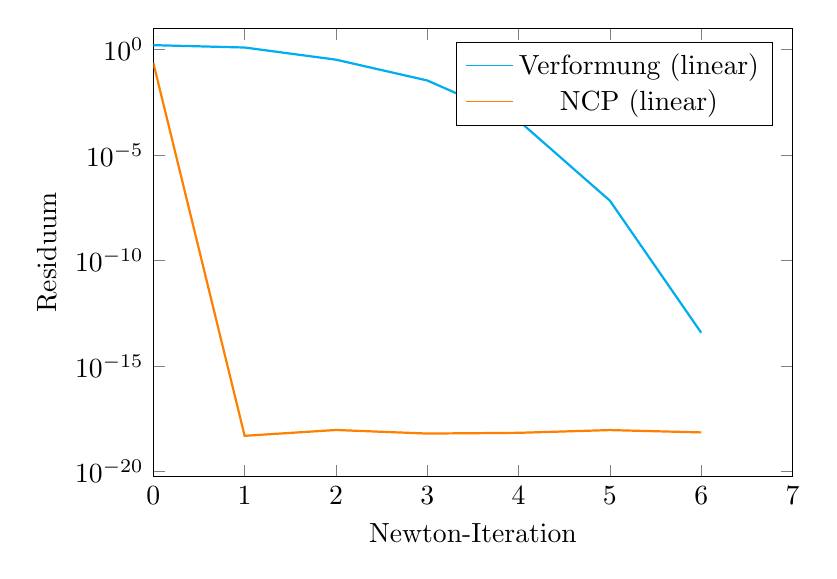
\begin{tikzpicture}[every plot/.append style={thick}] 
\begin{axis}[ 
label style={font=\normalsize}, 
xlabel={Newton-Iteration}, 
ylabel={Residuum}, 
xmin=0, xmax=7, 
ymode=log, 
ymin=0, ymax=10, 
width=0.8\textwidth, 
height=0.6\textwidth, 
legend pos=north east, 
legend style={cells={align=left}}, 
grid style=dashed, 
] 
\addplot[ 
color=cyan, 
] 
coordinates { 
(0, 1.58e+00)(1, 1.22e+00)(2, 3.24e-01)(3, 3.35e-02)(4, 4.21e-04)(5, 6.76e-08)(6, 3.76e-14)}; 
\addlegendentry{Verformung (linear)} 
\addplot[ 
color=orange, 
] 
coordinates { 
(0, 2.31e-01)(1, 4.94e-19)(2, 9.32e-19)(3, 6.31e-19)(4, 6.84e-19)(5, 9.23e-19)(6, 7.16e-19)}; 
\addlegendentry{NCP (linear)} 
\end{axis} 
\end{tikzpicture} 
\caption{Residuen des Stoffgesetzes 'Neo Hooke' mit Hinderniss 'Spitze' und 8450 Freiheitsgraden für die Verschiebung.} 
\label{fiq:NeoHooke_Spitze_level5} 
\end{figure} 
